%======================================================================
% MODULE 4: Testing and Verification of Cyber-Physical Systems
%
% Learning Objectives:
% After completing this module, students will be able to:
% - Explain why testing CPS is fundamentally different from testing discrete software
% - Choose appropriate testing levels (MIL, SIL, HIL) for different development phases
% - Write formal requirements using Signal Temporal Logic
% - Compute robustness values for STL specifications
% - Set up and run falsification experiments using optimization
% - Apply debugging techniques for embedded flight controllers
%======================================================================

\chapter{Introduction to CPS Testing}
\index{testing}

\section{Why Testing Cyber-Physical Systems is Hard}

Testing a cyber-physical system like a quadrotor flight controller is fundamentally different from testing traditional software. To understand why, consider the differences:

\textbf{Traditional software testing}: The program takes discrete inputs and produces discrete outputs. You can enumerate test cases, check outputs against expected values, and achieve meaningful coverage of the input space.

\textbf{CPS testing}: The controller interacts with continuous physical dynamics. Inputs are continuous signals (sensor readings over time), outputs are continuous signals (motor commands over time), and the behavior depends on differential equations that evolve in continuous time.

\begin{keyidea}[title=The Continuous State Space Problem]
A quadrotor's state includes position (3D), velocity (3D), orientation (4D quaternion), and angular velocity (3D)---at minimum 13 continuous variables. Each variable takes values from a continuous range. The space of possible trajectories is \textbf{uncountably infinite}.

Unlike discrete software where you might test all branches, you cannot test all possible flight trajectories. Testing must be strategic, focusing on scenarios most likely to reveal problems.
\end{keyidea}

\subsection{What Makes Quadrotor Testing Challenging}

\begin{enumerate}
    \item \textbf{Nonlinear dynamics}: Small changes in initial conditions can lead to dramatically different trajectories. A controller that works perfectly in one scenario may fail in a slightly different one.

    \item \textbf{Real-time constraints}: The controller must respond within milliseconds. A correct algorithm that runs too slowly is as bad as an incorrect one.

    \item \textbf{Environmental uncertainty}: Wind gusts, sensor noise, and battery voltage variations create disturbances that are impossible to predict exactly.

    \item \textbf{Coupled subsystems}: Attitude control affects position control; sensor fusion affects both. Bugs may only appear when subsystems interact.

    \item \textbf{Safety criticality}: A software crash on your laptop is annoying. A flight controller crash means a falling quadrotor---potential injury, property damage, or worse.
\end{enumerate}

\subsection{The Role of Models in Testing}

Since we cannot test exhaustively, we rely on \textbf{models} to:
\begin{itemize}
    \item Simulate the physical plant (quadrotor dynamics) without risking hardware
    \item Generate test scenarios systematically
    \item Specify requirements formally so they can be checked automatically
    \item Predict behavior in conditions we haven't explicitly tested
\end{itemize}

\begin{notebox}
The quality of testing is limited by the quality of models. A test that passes in simulation only means the \textit{model} of the quadrotor behaves correctly. Whether the \textit{real} quadrotor behaves the same depends on model fidelity---how accurately the model captures reality.
\end{notebox}

\section{Verification vs. Validation vs. Testing}

These terms are often confused. In the context of CPS development:

\begin{definition}[Verification]
\index{verification}
\textbf{Verification}\index{verification|textbf} asks: ``Did we build the system right?'' It checks that the implementation matches the specification. Formal verification uses mathematical proofs; testing-based verification uses systematic test cases.
\end{definition}

\begin{definition}[Validation]
\index{validation}
\textbf{Validation}\index{validation|textbf} asks: ``Did we build the right system?'' It checks that the specification captures what users actually need. A controller might perfectly meet its specification yet still be useless if the specification was wrong.
\end{definition}

\begin{definition}[Testing]
\textbf{Testing} executes the system with specific inputs and checks outputs against expected behavior. Testing can find bugs (show presence of errors) but cannot prove their absence---there's always another test case you haven't tried.
\end{definition}

\section{The Fundamental Limitation}

\begin{warningbox}
For hybrid systems (combining discrete software states with continuous physical dynamics), the problem of determining whether a given state is reachable is \textbf{undecidable}.

This means: No algorithm exists that can always determine, in finite time, whether a specification is satisfied for all possible inputs and initial conditions.
\end{warningbox}

This undecidability result has profound implications:
\begin{itemize}
    \item We cannot build a ``verify'' button that guarantees safety for arbitrary CPS
    \item Formal verification methods work only for restricted system classes
    \item For general CPS, we must rely on testing, which can never be complete
    \item Safety-critical systems require defense in depth: multiple complementary methods
\end{itemize}

Despite this limitation, we can still achieve high confidence through:
\begin{enumerate}
    \item \textbf{Formal methods} for critical subsystems that fit within decidable classes
    \item \textbf{Systematic testing} guided by formal specifications
    \item \textbf{Runtime monitoring} to detect violations during operation
    \item \textbf{Fail-safe mechanisms} to handle unexpected situations
\end{enumerate}

%======================================================================
\chapter{Development Process and Testing Levels}
%======================================================================

\section{The V-Model for CPS Development}
\index{V-model}

The V-model~\cite{forsberg2005visualizing}\index{V-model|textbf} is a development framework that maps each design phase to a corresponding testing phase:

\begin{center}
\begin{tikzpicture}[scale=0.9, every node/.style={font=\small}]
    % Left side - development (descending from top-left to center-bottom)
    \node[draw, rectangle, minimum width=3cm, minimum height=0.8cm] (req) at (0, 3) {Requirements};
    \node[draw, rectangle, minimum width=3cm, minimum height=0.8cm] (arch) at (2, 2) {Architecture};
    \node[draw, rectangle, minimum width=3cm, minimum height=0.8cm] (detail) at (4, 1) {Detailed Design};
    \node[draw, rectangle, minimum width=3cm, minimum height=0.8cm] (impl) at (6, 0) {Implementation};

    % Right side - testing (ascending from center-bottom to top-right)
    \node[draw, rectangle, minimum width=3cm, minimum height=0.8cm] (unit) at (8, 1) {Unit Testing};
    \node[draw, rectangle, minimum width=3cm, minimum height=0.8cm] (integ) at (10, 2) {Integration Testing};
    \node[draw, rectangle, minimum width=3cm, minimum height=0.8cm] (sys) at (12, 3) {System Testing};
    \node[draw, rectangle, minimum width=3cm, minimum height=0.8cm] (accept) at (14, 4) {Acceptance Testing};

    % Arrows down left
    \draw[-{Stealth}] (req.south east) -- (arch.north west);
    \draw[-{Stealth}] (arch.south east) -- (detail.north west);
    \draw[-{Stealth}] (detail.south east) -- (impl.north west);

    % Arrows up right
    \draw[-{Stealth}] (impl.north east) -- (unit.south west);
    \draw[-{Stealth}] (unit.north east) -- (integ.south west);
    \draw[-{Stealth}] (integ.north east) -- (sys.south west);
    \draw[-{Stealth}] (sys.north east) -- (accept.south west);

    % Horizontal arrows (traceability)
    \draw[dashed, -{Stealth}] (req.east) -- (accept.west) node[midway, above] {validates};
    \draw[dashed, -{Stealth}] (arch.east) -- (sys.west) node[midway, above] {verifies};
    \draw[dashed, -{Stealth}] (detail.east) -- (integ.west) node[midway, above] {verifies};
\end{tikzpicture}
\end{center}

For a quadrotor flight controller:
\begin{itemize}
    \item \textbf{Requirements}: ``The quadrotor shall maintain hover within 10 cm for 30 seconds''
    \item \textbf{Architecture}: Cascaded control (outer position loop, inner attitude loop)
    \item \textbf{Detailed Design}: PID gains, filter coefficients, task priorities
    \item \textbf{Implementation}: C code for FreeRTOS tasks
    \item \textbf{Unit Testing}: Test each function (e.g., quaternion multiplication)
    \item \textbf{Integration Testing}: Test subsystems together (sensor fusion + attitude control)
    \item \textbf{System Testing}: Test complete flight controller in simulation
    \item \textbf{Acceptance Testing}: Test on real hardware in flight
\end{itemize}

\section{Testing Levels for CPS}

CPS development uses specialized testing levels that progressively increase realism:

\subsection{Model-in-the-Loop (MIL) Testing}
\index{MIL (Model-in-the-Loop)}

In MIL testing\index{MIL (Model-in-the-Loop)|textbf}, both the controller and plant are \textbf{models} running in a simulation environment (e.g., MATLAB/Simulink).

\begin{center}
\begin{tikzpicture}[node distance=2cm]
    \node[draw, rectangle, minimum width=2.5cm, minimum height=1cm, fill=blue!10] (ctrl) {Controller Model};
    \node[draw, rectangle, minimum width=2.5cm, minimum height=1cm, fill=green!10, right=of ctrl] (plant) {Plant Model};

    \draw[-{Stealth}] (ctrl.east) -- (plant.west) node[midway, above] {$u$};
    \draw[-{Stealth}] (plant.south) -- ++(0, -0.5) -| (ctrl.south) node[near start, right] {$y$};

    \node[draw, dashed, fit=(ctrl)(plant), inner sep=10pt, label=above:Simulation Environment] {};
\end{tikzpicture}
\end{center}

\textbf{Advantages}:
\begin{itemize}
    \item Fast execution (faster than real-time possible)
    \item Complete observability of all internal states
    \item Easy to run thousands of test scenarios
    \item No risk to hardware
    \item Reproducible results
\end{itemize}

\textbf{Limitations}:
\begin{itemize}
    \item Controller model may not match actual implementation
    \item Plant model may not capture all physical effects
    \item No real-time constraints tested
\end{itemize}

\textbf{Use for quadrotors}: Early algorithm development, control design iteration, extensive parameter sweeps.

\subsection{Software-in-the-Loop (SIL) Testing}
\index{SIL (Software-in-the-Loop)}

In SIL testing\index{SIL (Software-in-the-Loop)|textbf}, the \textbf{actual controller code} runs on a development computer, interfacing with a plant model.

\begin{center}
\begin{tikzpicture}[node distance=2cm]
    \node[draw, rectangle, minimum width=2.5cm, minimum height=1cm, fill=blue!30] (ctrl) {Controller Code};
    \node[draw, rectangle, minimum width=2.5cm, minimum height=1cm, fill=green!10, right=of ctrl] (plant) {Plant Model};

    \draw[-{Stealth}] (ctrl.east) -- (plant.west) node[midway, above] {$u$};
    \draw[-{Stealth}] (plant.south) -- ++(0, -0.5) -| (ctrl.south) node[near start, right] {$y$};

    \node[draw, dashed, fit=(ctrl)(plant), inner sep=10pt, label=above:Development Computer] {};
\end{tikzpicture}
\end{center}

\textbf{Advantages}:
\begin{itemize}
    \item Tests actual implementation (same C code as embedded target)
    \item Can detect implementation bugs (overflow, precision loss)
    \item Still fast and reproducible
    \item Can use debugging tools (breakpoints, memory inspection)
\end{itemize}

\textbf{Limitations}:
\begin{itemize}
    \item Different processor architecture than target (x86 vs ARM)
    \item No real-time scheduling tested
    \item No hardware peripherals (I2C, SPI, PWM)
\end{itemize}

\textbf{Use for quadrotors}: Testing control algorithms after porting to C, verifying numerical correctness, debugging logic errors.

\subsection{Processor-in-the-Loop (PIL) Testing}

In PIL testing, the controller code runs on the \textbf{actual target processor}, but the plant is still simulated on a host computer.

\begin{center}
\begin{tikzpicture}[node distance=2.5cm]
    \node[draw, rectangle, minimum width=2.5cm, minimum height=1cm, fill=blue!50] (ctrl) {Controller Code};
    \node[draw, rectangle, minimum width=2.5cm, minimum height=1cm, fill=green!10, right=of ctrl] (plant) {Plant Model};

    \draw[-{Stealth}] (ctrl.east) -- (plant.west) node[midway, above] {$u$ (serial)};
    \draw[-{Stealth}] (plant.south) -- ++(0, -0.5) -| (ctrl.south) node[near start, right] {$y$ (serial)};

    \node[draw, dashed, fit=(ctrl), inner sep=5pt, label=below:Embedded Target] {};
    \node[draw, dashed, fit=(plant), inner sep=5pt, label=below:Host Computer] {};
\end{tikzpicture}
\end{center}

\textbf{Advantages}:
\begin{itemize}
    \item Tests on actual target processor (correct instruction set, FPU behavior)
    \item Reveals architecture-specific bugs (endianness, alignment)
    \item Can measure actual execution times
\end{itemize}

\textbf{Limitations}:
\begin{itemize}
    \item Communication overhead slows testing
    \item Still no real hardware peripherals
    \item Real-time behavior may be affected by communication
\end{itemize}

\subsection{Hardware-in-the-Loop (HIL) Testing}
\index{HIL (Hardware-in-the-Loop)}

In HIL testing\index{HIL (Hardware-in-the-Loop)|textbf}, the complete embedded system (controller + hardware interfaces) runs in real-time, but the plant is simulated by specialized real-time hardware.

\begin{center}
\begin{tikzpicture}[node distance=2.5cm]
    \node[draw, rectangle, minimum width=2.8cm, minimum height=1.2cm, fill=blue!50] (ctrl) {Flight Controller};
    \node[draw, rectangle, minimum width=2.8cm, minimum height=1.2cm, fill=green!30, right=of ctrl] (plant) {Real-Time Simulator};

    \draw[-{Stealth}] (ctrl.east) -- (plant.west) node[midway, above] {PWM signals};
    \draw[-{Stealth}] (plant.south) -- ++(0, -0.7) -| (ctrl.south) node[near start, right] {Sensor signals};

    \node[draw, dashed, fit=(ctrl), inner sep=5pt, label=below:Actual Hardware] {};
    \node[draw, dashed, fit=(plant), inner sep=5pt, label=below:Real-Time Target] {};
\end{tikzpicture}
\end{center}

\textbf{Advantages}:
\begin{itemize}
    \item Tests complete system including hardware interfaces
    \item Real-time behavior tested accurately
    \item Can test failure modes (sensor disconnect, actuator saturation)
    \item Safe testing of dangerous scenarios
\end{itemize}

\textbf{Limitations}:
\begin{itemize}
    \item Expensive real-time simulation hardware required
    \item Slower test execution (real-time only)
    \item Plant model fidelity still limits realism
    \item Cannot test all physical effects (vibration, temperature)
\end{itemize}

\textbf{Use for quadrotors}: Testing complete flight controller with actual sensor interfaces, testing failsafe behavior, regression testing before flight.

\subsection{Vehicle-in-the-Loop (VIL) Testing}

In VIL testing, the actual vehicle operates in a controlled environment, possibly with some simulated elements.

\textbf{Examples}:
\begin{itemize}
    \item Quadrotor on a test stand (constrained motion, safe if control fails)
    \item Flight in a netted arena with motion capture
    \item Outdoor flight with geofencing
\end{itemize}

\textbf{Advantages}:
\begin{itemize}
    \item Tests real physics, real sensors, real actuators
    \item Reveals effects not captured in simulation
    \item Final validation before deployment
\end{itemize}

\textbf{Limitations}:
\begin{itemize}
    \item Risk to hardware (and potentially people)
    \item Slow and expensive
    \item Not reproducible (environmental variations)
    \item Limited ability to test extreme scenarios
\end{itemize}

\section{Choosing the Right Testing Level}

\begin{keyidea}[title=The Testing Pyramid]
Most testing should happen at lower levels (MIL, SIL) where it's fast and cheap. Higher levels (HIL, VIL) are used selectively for integration and final validation.

\begin{center}
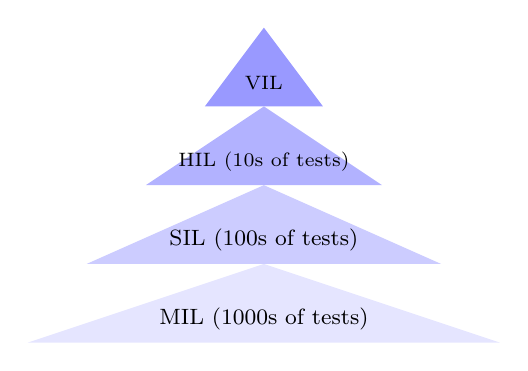
\begin{tikzpicture}
    % Wider pyramid to accommodate text labels
    \fill[blue!10] (-1,0) -- (5,0) -- (2,1) -- cycle;
    \fill[blue!20] (-0.25,1) -- (4.25,1) -- (2,2) -- cycle;
    \fill[blue!30] (0.5,2) -- (3.5,2) -- (2,3) -- cycle;
    \fill[blue!40] (1.25,3) -- (2.75,3) -- (2,4) -- cycle;

    \node[font=\footnotesize] at (2, 0.3) {MIL (1000s of tests)};
    \node[font=\footnotesize] at (2, 1.3) {SIL (100s of tests)};
    \node[font=\scriptsize] at (2, 2.3) {HIL (10s of tests)};
    \node[font=\scriptsize] at (2, 3.3) {VIL};
\end{tikzpicture}
\end{center}
\end{keyidea}

\begin{center}
\begin{tabular}{lcccc}
\toprule
\textbf{Aspect} & \textbf{MIL} & \textbf{SIL} & \textbf{HIL} & \textbf{VIL} \\
\midrule
Execution speed & 100$\times$ RT & 10$\times$ RT & 1$\times$ RT & 1$\times$ RT \\
Tests per day & 10,000+ & 1,000+ & 100 & 10 \\
Hardware needed & None & None & RT simulator & Vehicle \\
Risk & None & None & Low & Medium-High \\
Realism & Low & Medium & High & Highest \\
Debugging ease & Easy & Easy & Medium & Hard \\
\bottomrule
\end{tabular}
\end{center}

%======================================================================
\chapter{Requirements for Flight Controllers}
%======================================================================

\section{From Informal to Formal Requirements}

Requirements typically start as informal natural language statements from stakeholders:
\begin{itemize}
    \item ``The drone should fly stably''
    \item ``It should respond quickly to commands''
    \item ``It must not fly outside the designated area''
    \item ``Battery should last at least 5 minutes''
\end{itemize}

These informal requirements must be refined into \textbf{formal, testable specifications}. The process involves:
\begin{enumerate}
    \item \textbf{Clarification}: What exactly does ``stably'' mean? What is ``quickly''?
    \item \textbf{Quantification}: Add numerical bounds and tolerances
    \item \textbf{Formalization}: Express in a language that can be checked automatically
\end{enumerate}

\begin{example}[Refining a Requirement]
\textbf{Informal}: ``The drone should fly stably''

\textbf{Clarified}: ``The attitude angles should not exceed safe limits''

\textbf{Quantified}: ``Roll and pitch angles shall remain within $\pm30°$ during normal flight''

\textbf{Formalized} (in Signal Temporal Logic):
\[
\Box_{[0,T]}\left( |\phi| < 30° \land |\theta| < 30° \right)
\]
where $\phi$ is roll, $\theta$ is pitch, and $T$ is the flight duration.
\end{example}

\section{Categories of Flight Controller Requirements}

\subsection{Safety Requirements}

Safety requirements define conditions that must \textbf{never} be violated:

\begin{center}
\begin{tabular}{p{4cm}p{7cm}}
\toprule
\textbf{Requirement} & \textbf{Formalization} \\
\midrule
Attitude limits & $\Box_{[0,T]}(|\phi| < \phi_{max} \land |\theta| < \theta_{max})$ \\
Altitude ceiling & $\Box_{[0,T]}(z < z_{max})$ \\
Geofencing & $\Box_{[0,T]}(x_{min} < x < x_{max} \land y_{min} < y < y_{max})$ \\
Motor limits & $\Box_{[0,T]}(0 \leq \omega_i \leq \omega_{max})$ for all motors \\
Angular rate limits & $\Box_{[0,T]}(|\dot{\phi}| < \dot{\phi}_{max})$ \\
\bottomrule
\end{tabular}
\end{center}

\subsection{Performance Requirements}

Performance requirements specify how well the system should respond:

\begin{center}
\begin{tabular}{p{4cm}p{7cm}}
\toprule
\textbf{Requirement} & \textbf{Formalization} \\
\midrule
Settling time & $\Diamond_{[0, t_s]}(|e| < \epsilon) \land \Box_{[t_s, T]}(|e| < \epsilon)$ \\
Overshoot & $\Box_{[0,T]}(y < y_{ref} \cdot (1 + OS_{max}))$ \\
Steady-state error & $\Box_{[t_s, T]}(|e| < e_{ss})$ \\
Rise time & $\Diamond_{[0, t_r]}(y > 0.9 \cdot y_{ref})$ \\
\bottomrule
\end{tabular}
\end{center}

\begin{example}[Settling Time Requirement]
``After a step command, the position error shall be less than 5 cm within 2 seconds and remain below 5 cm thereafter.''

\[
\Diamond_{[0, 2]}\left( \|p - p_{ref}\| < 0.05 \right) \land \Box_{[2, T]}\left( \|p - p_{ref}\| < 0.05 \right)
\]

This requires the error to \textit{eventually} (within 2 seconds) become small, and then \textit{always} remain small.
\end{example}

\subsection{Robustness Requirements}

Robustness requirements specify that the system should work under disturbances:

\begin{itemize}
    \item ``The controller shall maintain hover within 20 cm under wind gusts up to 5 m/s''
    \item ``The system shall remain stable with up to 10\% mass uncertainty''
    \item ``Position accuracy shall be maintained with sensor noise up to $\sigma = 0.1$ m''
\end{itemize}

These are tested by applying disturbances during simulation and checking that safety/performance requirements still hold.

\subsection{Timing Requirements}

For real-time systems, timing is part of correctness:

\begin{itemize}
    \item ``Control loop shall execute at 500 Hz with jitter less than 100 $\mu$s''
    \item ``Sensor data shall be processed within 1 ms of arrival''
    \item ``Failsafe shall activate within 50 ms of communication loss''
\end{itemize}

\section{Requirements for the Crazyflie Project}

For the course project, consider requirements such as:

\textbf{Attitude Control}:
\begin{enumerate}
    \item Roll/pitch angles shall remain within $\pm 45°$ during all maneuvers
    \item Given a step change in attitude reference, the attitude error shall settle to within $2°$ in less than 0.5 seconds
    \item Attitude control shall remain stable with up to 20\% variation in moment of inertia
\end{enumerate}

\textbf{Position Control}:
\begin{enumerate}
    \item Position shall remain within a 2 m $\times$ 2 m $\times$ 2 m box at all times
    \item Hover position error shall be less than 10 cm in steady state
    \item After a position step command, the quadrotor shall reach within 15 cm of target in less than 3 seconds
\end{enumerate}

\textbf{Failsafe}:
\begin{enumerate}
    \item If communication is lost for more than 500 ms, motors shall be cut
    \item If attitude exceeds $60°$, motors shall be cut
    \item If battery voltage drops below 3.0 V per cell, the quadrotor shall land
\end{enumerate}

%======================================================================
\chapter{Signal Temporal Logic (STL)}
\index{STL (Signal Temporal Logic)}
%======================================================================

\section{Why Temporal Logic for CPS}

Traditional testing checks: ``Is the output correct at this instant?''

For CPS, we need to check properties over \textbf{time}: ``Does the signal stay below the limit for the entire interval?'' ``Does it eventually reach the target?'' ``Does event A always precede event B?''

\textbf{Signal Temporal Logic (STL)}~\cite{maler2004monitoring}\index{STL (Signal Temporal Logic)|textbf} provides a formal language to express such temporal properties over continuous-time signals.

\section{Predicates Over Continuous Signals}

The building blocks of STL are \textbf{predicates}---conditions on signal values at a particular time:

\begin{definition}[Predicate]
A predicate $\mu$ is a condition of the form $f(x(t)) \sim c$ where:
\begin{itemize}
    \item $x(t)$ is the signal (e.g., position, velocity, attitude)
    \item $f$ is a function of the signal
    \item $\sim$ is a comparison operator ($<$, $\leq$, $>$, $\geq$, $=$)
    \item $c$ is a constant threshold
\end{itemize}
\end{definition}

\begin{example}[Predicates for Quadrotor Signals]
\begin{align*}
\mu_1 &: z < 10 && \text{``altitude is below 10 meters''} \\
\mu_2 &: \|p - p_{ref}\| < 0.1 && \text{``position error is less than 10 cm''} \\
\mu_3 &: |\phi| < 30° && \text{``roll angle magnitude is less than 30 degrees''} \\
\mu_4 &: \omega_1 > 1000 && \text{``motor 1 speed exceeds 1000 RPM''} \\
\mu_5 &: v_z > 0 && \text{``quadrotor is ascending''}
\end{align*}
\end{example}

A predicate $\mu$ is either \texttt{True} or \texttt{False} at each time instant $t$, depending on the signal value $x(t)$.

\section{Boolean Operators}

Predicates can be combined using standard Boolean operators:

\begin{center}
\begin{tabular}{lll}
\toprule
\textbf{Operator} & \textbf{Symbol} & \textbf{Meaning} \\
\midrule
Negation & $\neg \mu$ & NOT $\mu$ \\
Conjunction & $\mu_1 \land \mu_2$ & $\mu_1$ AND $\mu_2$ \\
Disjunction & $\mu_1 \lor \mu_2$ & $\mu_1$ OR $\mu_2$ \\
Implication & $\mu_1 \Rightarrow \mu_2$ & IF $\mu_1$ THEN $\mu_2$ (equivalent to $\neg\mu_1 \lor \mu_2$) \\
\bottomrule
\end{tabular}
\end{center}

\begin{example}[Combined Predicates]
``The quadrotor is in a safe attitude'':
\[
\text{safe\_attitude} = (|\phi| < 45°) \land (|\theta| < 45°)
\]

``Either hovering or moving slowly'':
\[
(\|v\| < 0.1) \lor (\|v\| < 1.0 \land z < 2)
\]
\end{example}

\section{The Always Operator ($\Box$)}

\begin{definition}[Always / Globally]
$\Box_{[a,b]} \varphi$ means: formula $\varphi$ holds at \textbf{every} time instant in the interval $[t+a, t+b]$, where $t$ is the current time.
\end{definition}

\begin{center}
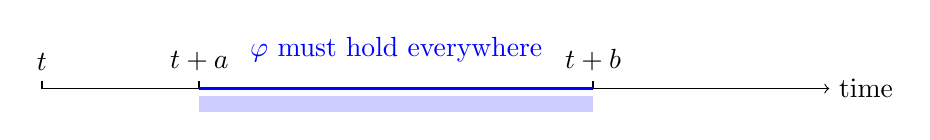
\begin{tikzpicture}
    \draw[->] (0,0) -- (10,0) node[right] {time};
    \draw[thick] (0,0) -- (0,0.1) node[above] {$t$};
    \draw[thick] (2,0) -- (2,0.1) node[above] {$t+a$};
    \draw[thick] (7,0) -- (7,0.1) node[above] {$t+b$};

    \draw[very thick, blue] (2,0) -- (7,0);
    \node[blue] at (4.5, 0.5) {$\varphi$ must hold everywhere};

    \fill[blue!20] (2,-0.3) rectangle (7,-0.1);
\end{tikzpicture}
\end{center}

\begin{example}[Always Operator]
``Altitude stays below 10 m for the entire flight (0 to T seconds)'':
\[
\Box_{[0,T]}(z < 10)
\]

``For the next 5 seconds, attitude remains safe'':
\[
\Box_{[0,5]}(|\phi| < 45° \land |\theta| < 45°)
\]

``From time 2s to 10s, position error is small'':
\[
\Box_{[2,10]}(\|p - p_{ref}\| < 0.1)
\]
\end{example}

\textbf{Intuition}: $\Box_{[a,b]}$ is like a \texttt{for all} quantifier over time. The formula must be true at every moment in the interval.

\section{The Eventually Operator ($\Diamond$)}

\begin{definition}[Eventually / Finally]
$\Diamond_{[a,b]} \varphi$ means: formula $\varphi$ holds at \textbf{some} time instant in the interval $[t+a, t+b]$.
\end{definition}

\begin{center}
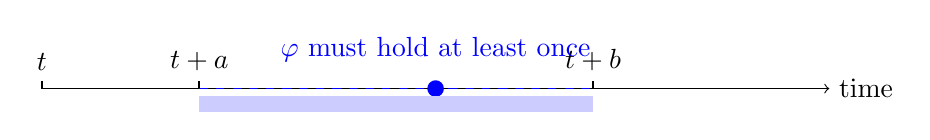
\begin{tikzpicture}
    \draw[->] (0,0) -- (10,0) node[right] {time};
    \draw[thick] (0,0) -- (0,0.1) node[above] {$t$};
    \draw[thick] (2,0) -- (2,0.1) node[above] {$t+a$};
    \draw[thick] (7,0) -- (7,0.1) node[above] {$t+b$};

    \draw[dashed, blue] (2,0) -- (7,0);
    \fill[blue] (5,0) circle (3pt);
    \node[blue] at (5, 0.5) {$\varphi$ must hold at least once};

    \fill[blue!20] (2,-0.3) rectangle (7,-0.1);
\end{tikzpicture}
\end{center}

\begin{example}[Eventually Operator]
``The quadrotor reaches the target within 5 seconds'':
\[
\Diamond_{[0,5]}(\|p - p_{ref}\| < 0.1)
\]

``At some point between 2s and 4s, the quadrotor is descending'':
\[
\Diamond_{[2,4]}(v_z < 0)
\]

``Eventually (within the mission time), the quadrotor lands'':
\[
\Diamond_{[0,T]}(z < 0.1 \land \|v\| < 0.1)
\]
\end{example}

\textbf{Intuition}: $\Diamond_{[a,b]}$ is like an \texttt{exists} quantifier over time. The formula needs to be true at just one moment in the interval.

\textbf{Relationship}: $\Diamond_{[a,b]} \varphi \equiv \neg \Box_{[a,b]} \neg\varphi$ (eventually $\varphi$ means it's not always not-$\varphi$).

\section{The Until Operator ($\mathcal{U}$)}

\begin{definition}[Until]
$\varphi_1 \mathcal{U}_{[a,b]} \varphi_2$ means: $\varphi_1$ holds continuously until $\varphi_2$ becomes true, and $\varphi_2$ becomes true at some time in $[t+a, t+b]$.
\end{definition}

\begin{center}
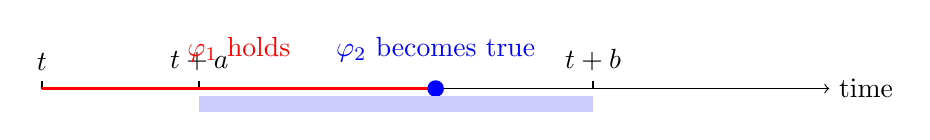
\begin{tikzpicture}
    \draw[->] (0,0) -- (10,0) node[right] {time};
    \draw[thick] (0,0) -- (0,0.1) node[above] {$t$};
    \draw[thick] (2,0) -- (2,0.1) node[above] {$t+a$};
    \draw[thick] (7,0) -- (7,0.1) node[above] {$t+b$};

    \draw[very thick, red] (0,0) -- (5,0);
    \node[red] at (2.5, 0.5) {$\varphi_1$ holds};

    \fill[blue] (5,0) circle (3pt);
    \node[blue] at (5, 0.5) {$\varphi_2$ becomes true};

    \fill[blue!20] (2,-0.3) rectangle (7,-0.1);
\end{tikzpicture}
\end{center}

\begin{example}[Until Operator]
``The quadrotor maintains altitude until it receives a land command'':
\[
(|z - z_{hover}| < 0.1) \mathcal{U}_{[0,T]} (\text{land\_cmd} = 1)
\]

``Attitude remains level until the waypoint is reached'':
\[
(|\phi| < 5° \land |\theta| < 5°) \mathcal{U}_{[0,10]} (\|p - p_{wp}\| < 0.2)
\]
\end{example}

\section{Combining Operators}

Complex requirements often require nested temporal operators:

\begin{example}[Settling Time Specification]
``After a step command at $t=0$, the error shall eventually become small and then always remain small'':
\[
\Diamond_{[0,2]} \Box_{[0,\infty)} (\|e\| < 0.05)
\]

This means: at some time within 2 seconds, a point is reached after which the error is always small.
\end{example}

\begin{example}[Response to Disturbance]
``If a wind gust occurs, the position error may temporarily increase but shall return to normal within 3 seconds'':
\[
\Box_{[0,T]} \left( (\text{gust} > 2) \Rightarrow \Diamond_{[0,3]}(\|e_p\| < 0.1) \right)
\]

Whenever a gust exceeds 2 m/s, the system must recover within 3 seconds.
\end{example}

\begin{example}[Safety with Recovery]
``Attitude angles shall always remain safe, and if they exceed 20°, they must return below 10° within 1 second'':
\[
\Box_{[0,T]}(|\phi| < 45°) \land \Box_{[0,T]}\left( (|\phi| > 20°) \Rightarrow \Diamond_{[0,1]}(|\phi| < 10°) \right)
\]
\end{example}

\section{Common STL Specification Patterns}

\begin{center}
\begin{tabular}{p{3.5cm}p{4cm}p{4.5cm}}
\toprule
\textbf{Pattern} & \textbf{Informal} & \textbf{STL} \\
\midrule
Invariance & Always safe & $\Box_{[0,T]} \varphi$ \\
Reachability & Eventually reach goal & $\Diamond_{[0,T]} \varphi$ \\
Stability & Reach and stay & $\Diamond_{[0,t_s]} \Box_{[0,\infty)} \varphi$ \\
Bounded response & If $\varphi_1$ then $\varphi_2$ within $\tau$ & $\Box_{[0,T]}(\varphi_1 \Rightarrow \Diamond_{[0,\tau]}\varphi_2)$ \\
Recurrence & Keep returning to $\varphi$ & $\Box_{[0,T]} \Diamond_{[0,\tau]} \varphi$ \\
\bottomrule
\end{tabular}
\end{center}

%======================================================================
\chapter{Quantitative Semantics: Robustness}
\index{robustness}
%======================================================================

\section{From Boolean to Quantitative}

STL formulas are either satisfied or violated---a Boolean outcome. However, for testing and optimization, we need more information:
\begin{itemize}
    \item \textbf{How much margin} do we have before violation?
    \item Is a trajectory that barely satisfies the spec as good as one with large margin?
    \item How can we guide optimization to find violations?
\end{itemize}

\textbf{Robustness}~\cite{donze2010robust,fainekos2009robustness} extends STL with quantitative semantics: instead of just True/False, we compute a real number indicating how strongly the formula is satisfied or violated.

\begin{keyidea}[title=Robustness Semantics]
The robustness value $\rho(\varphi, x, t)$ of formula $\varphi$ for signal $x$ at time $t$ is:
\begin{itemize}
    \item \textbf{Positive} if $\varphi$ is satisfied (larger = more margin)
    \item \textbf{Negative} if $\varphi$ is violated (more negative = worse violation)
    \item \textbf{Zero} at the boundary between satisfaction and violation
\end{itemize}

Sign of robustness determines satisfaction: $\rho > 0 \Leftrightarrow$ formula satisfied.
\end{keyidea}

\section{Robustness of Predicates}

For a predicate $\mu : f(x) < c$, the robustness is simply the distance to the threshold:
\[
\rho(\mu, x, t) = c - f(x(t))
\]

\begin{example}[Predicate Robustness]
For $\mu : z < 10$ (altitude below 10 m):
\begin{itemize}
    \item If $z(t) = 7$: $\rho = 10 - 7 = 3$ (3 meters of margin)
    \item If $z(t) = 9.5$: $\rho = 10 - 9.5 = 0.5$ (barely satisfied)
    \item If $z(t) = 12$: $\rho = 10 - 12 = -2$ (violated by 2 meters)
\end{itemize}
\end{example}

For predicates with $>$: $\rho(f(x) > c, x, t) = f(x(t)) - c$.

\section{Robustness of Boolean Operators}

The robustness of compound formulas is computed recursively:

\begin{align}
\rho(\neg\varphi, x, t) &= -\rho(\varphi, x, t) \\
\rho(\varphi_1 \land \varphi_2, x, t) &= \min(\rho(\varphi_1, x, t), \rho(\varphi_2, x, t)) \\
\rho(\varphi_1 \lor \varphi_2, x, t) &= \max(\rho(\varphi_1, x, t), \rho(\varphi_2, x, t))
\end{align}

\textbf{Intuition}:
\begin{itemize}
    \item \textbf{Negation}: Flips the sign (what was margin becomes violation)
    \item \textbf{AND}: The conjunction is only as robust as its weakest part (minimum)
    \item \textbf{OR}: The disjunction is as robust as its strongest part (maximum)
\end{itemize}

\begin{example}[Compound Robustness]
For $\varphi = (z < 10) \land (|\phi| < 45°)$:

If $z = 8$ and $|\phi| = 30°$:
\begin{itemize}
    \item $\rho(z < 10) = 10 - 8 = 2$
    \item $\rho(|\phi| < 45°) = 45 - 30 = 15$
    \item $\rho(\varphi) = \min(2, 15) = 2$
\end{itemize}

The overall robustness is limited by altitude (the weaker constraint).
\end{example}

\section{Robustness of Temporal Operators}

\begin{align}
\rho(\Box_{[a,b]}\varphi, x, t) &= \min_{\tau \in [t+a, t+b]} \rho(\varphi, x, \tau) \\
\rho(\Diamond_{[a,b]}\varphi, x, t) &= \max_{\tau \in [t+a, t+b]} \rho(\varphi, x, \tau)
\end{align}

\textbf{Intuition}:
\begin{itemize}
    \item \textbf{Always}: Must hold at every instant, so robustness is the minimum over time
    \item \textbf{Eventually}: Must hold at some instant, so robustness is the maximum over time
\end{itemize}

\begin{example}[Temporal Robustness]
Consider $\varphi = \Box_{[0,5]}(z < 10)$ with altitude trajectory:
\[
z(t) = 5 + 2\sin(t)
\]

The altitude oscillates between 3 and 7. At each instant:
\[
\rho(z < 10, z, t) = 10 - z(t) = 5 - 2\sin(t)
\]

The minimum occurs when $\sin(t) = 1$: $\rho_{min} = 5 - 2 = 3$.

Therefore: $\rho(\Box_{[0,5]}(z < 10)) = 3$.

The trajectory satisfies the spec with 3 meters of margin (the closest approach to the limit).
\end{example}

\section{Geometric Interpretation}

\begin{center}
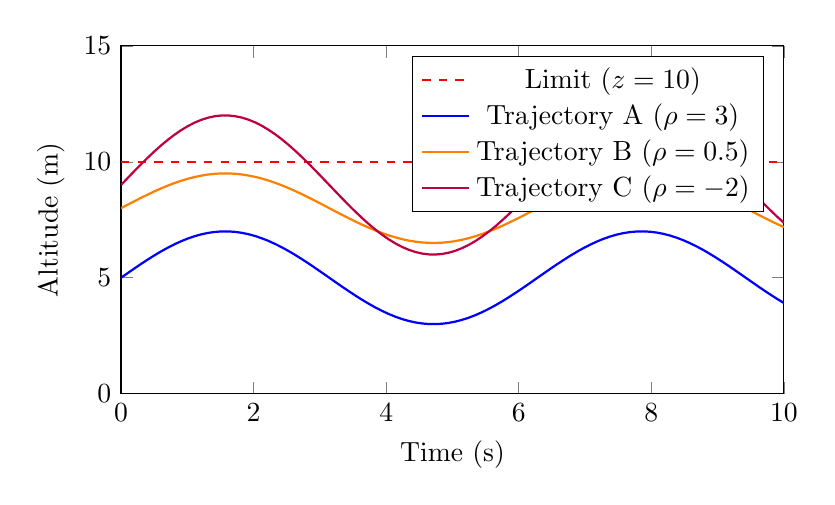
\begin{tikzpicture}
    \begin{axis}[
        width=10cm, height=6cm,
        xlabel={Time (s)}, ylabel={Altitude (m)},
        xmin=0, xmax=10, ymin=0, ymax=15,
        legend pos=north east
    ]
    % Threshold
    \addplot[red, thick, dashed, domain=0:10] {10};
    \addlegendentry{Limit ($z=10$)}

    % Trajectory 1 - good margin
    \addplot[blue, thick, domain=0:10, samples=100] {5 + 2*sin(deg(x))};
    \addlegendentry{Trajectory A ($\rho=3$)}

    % Trajectory 2 - close to limit
    \addplot[orange, thick, domain=0:10, samples=100] {8 + 1.5*sin(deg(x))};
    \addlegendentry{Trajectory B ($\rho=0.5$)}

    % Trajectory 3 - violation
    \addplot[purple, thick, domain=0:10, samples=100] {9 + 3*sin(deg(x))};
    \addlegendentry{Trajectory C ($\rho=-2$)}

    \end{axis}
\end{tikzpicture}
\end{center}

The robustness measures the \textbf{vertical distance} between the trajectory and the constraint boundary at the closest point:
\begin{itemize}
    \item Trajectory A: Always well below limit, robustness = +3
    \item Trajectory B: Comes close to limit, robustness = +0.5
    \item Trajectory C: Exceeds limit, robustness = -2
\end{itemize}

\section{Why Robustness Enables Optimization}

Traditional Boolean satisfaction provides no gradient information:
\begin{itemize}
    \item Trajectory that violates by 0.01 m: \texttt{False}
    \item Trajectory that violates by 10 m: \texttt{False}
\end{itemize}

Robustness provides a \textbf{continuous objective function}:
\begin{itemize}
    \item Trajectory that violates by 0.01 m: $\rho = -0.01$
    \item Trajectory that violates by 10 m: $\rho = -10$
\end{itemize}

This allows optimization algorithms to:
\begin{enumerate}
    \item Distinguish between ``almost satisfies'' and ``badly violates''
    \item Follow the gradient toward violations (for falsification)
    \item Quantify how much design margin exists
\end{enumerate}

%======================================================================
\chapter{Falsification: Testing as Optimization}
\index{falsification}
%======================================================================

Falsification-based testing uses optimization to systematically search for specification violations. For foundational work on this approach, see Donzé~\cite{donze2010breach} and Annpureddy et al.~\cite{annpureddy2011s}.

\section{The Falsification Problem}

\begin{definition}[Falsification]
\index{falsification|textbf}
Given:
\begin{enumerate}
    \item A \textbf{system model} $M$ (plant + controller)
    \item A \textbf{specification} $\varphi$ (in STL)
    \item A \textbf{set of test inputs} $\mathcal{K}$ (disturbances, initial conditions, parameters)
\end{enumerate}

\textbf{Find}: An input $k \in \mathcal{K}$ such that the resulting trajectory $x = M(k)$ violates the specification, i.e., $\rho(\varphi, x, 0) < 0$.
\end{definition}

Falsification is formulated as an \textbf{optimization problem}:
\[
\min_{k \in \mathcal{K}} \rho(\varphi, M(k), 0)
\]

If the minimum is negative, we have found a counterexample (falsified the spec). If extensive search fails to find negative robustness, we gain confidence (but not proof) that the spec is satisfied.

\begin{keyidea}[title=Testing as Optimization]
Instead of random testing or manual test case design, falsification uses optimization to \textbf{systematically search} for violations. The robustness function guides the search toward the most problematic inputs.
\end{keyidea}

\section{Test Input Parameterization}

The test inputs $k$ define the ``scenario'' being tested. For a quadrotor, inputs might include:

\textbf{Initial conditions}:
\begin{itemize}
    \item Initial position offset: $p_0 \in [-0.5, 0.5]^3$ m
    \item Initial velocity: $v_0 \in [-1, 1]^3$ m/s
    \item Initial attitude error: $\phi_0, \theta_0 \in [-10°, 10°]$
\end{itemize}

\textbf{Disturbance signals} (e.g., wind):
\begin{itemize}
    \item Time-varying signals are parameterized using \textbf{control points}
    \item Interpolation between control points creates smooth signals
\end{itemize}

\begin{example}[Wind Gust Parameterization]
A wind gust signal $w(t)$ over 10 seconds can be parameterized by 5 control points:
\[
k = [w_0, w_1, w_2, w_3, w_4, t_1, t_2, t_3, t_4]
\]
where $w_i$ is the wind speed at time $t_i$, with linear interpolation between points.

\begin{center}
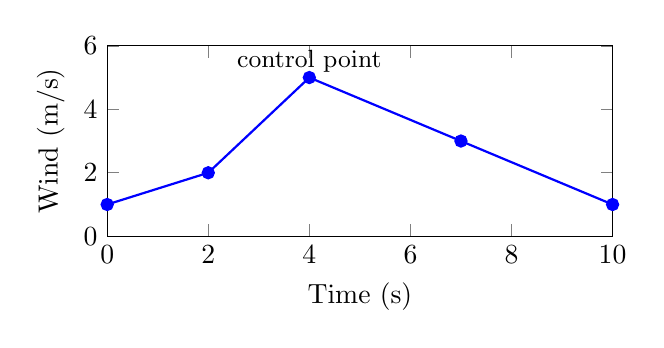
\begin{tikzpicture}
    \begin{axis}[
        width=8cm, height=4cm,
        xlabel={Time (s)}, ylabel={Wind (m/s)},
        xmin=0, xmax=10, ymin=0, ymax=6
    ]
    \addplot[blue, thick, mark=*] coordinates {
        (0, 1) (2, 2) (4, 5) (7, 3) (10, 1)
    };
    \node at (axis cs:4,5.5) {\small control point};
    \end{axis}
\end{tikzpicture}
\end{center}

The optimizer searches over the 9-dimensional parameter space to find wind patterns that cause violations.
\end{example}

\textbf{Reference signals}:
\begin{itemize}
    \item Waypoint positions
    \item Trajectory aggressiveness
    \item Command timing
\end{itemize}

\section{The Optimization Landscape}

The function $f(k) = \rho(\varphi, M(k), 0)$ defines a landscape over the parameter space:

\begin{itemize}
    \item \textbf{Valleys} (negative regions) represent violations
    \item \textbf{Hills} (positive regions) represent satisfaction
    \item \textbf{Zero crossings} are the boundaries
\end{itemize}

\begin{warningbox}
The robustness landscape is typically:
\begin{itemize}
    \item \textbf{Non-convex}: Multiple local minima
    \item \textbf{Non-smooth}: Discontinuities from mode switches, saturation
    \item \textbf{High-dimensional}: Many parameters
    \item \textbf{Expensive to evaluate}: Each point requires a full simulation
\end{itemize}

Gradient-based optimization often fails. We need gradient-free global optimization methods.
\end{warningbox}

\section{Gradient-Free Optimization Methods}

\subsection{CMA-ES (Covariance Matrix Adaptation Evolution Strategy)}

CMA-ES maintains a population of candidate solutions and adapts the search distribution based on which candidates perform well.

\textbf{Key idea}: Learn the shape of the objective function by tracking correlations between parameters in successful candidates.

\textbf{Strengths}: Good for non-convex, high-dimensional problems; self-adapting step size.

\subsection{Simulated Annealing}

Inspired by metallurgical annealing, this method accepts worse solutions with decreasing probability as the ``temperature'' cools.

\textbf{Key idea}: Early exploration accepts bad moves to escape local minima; later exploitation focuses on refinement.

\subsection{Nelder-Mead (Simplex Method)}

Maintains a simplex (triangle in 2D, tetrahedron in 3D) and iteratively moves it toward the minimum through reflection, expansion, and contraction operations.

\textbf{Strengths}: Simple, no hyperparameters, works well in low dimensions.

\textbf{Weaknesses}: Can get stuck in local minima; slow in high dimensions.

\subsection{Bayesian Optimization}

Builds a probabilistic model (Gaussian Process) of the objective function and uses it to decide where to sample next.

\textbf{Key idea}: Balance \textbf{exploitation} (sample where model predicts low values) with \textbf{exploration} (sample where model is uncertain).

\textbf{Strengths}: Sample-efficient (finds minima with fewer simulations); provides uncertainty estimates.

\textbf{Weaknesses}: Computational overhead for large datasets; GP scales poorly with dimensions.

\begin{center}
\begin{tabular}{lccc}
\toprule
\textbf{Method} & \textbf{Sample Efficiency} & \textbf{Scalability} & \textbf{Local Minima} \\
\midrule
CMA-ES & Medium & Good & Good escape \\
Simulated Annealing & Low & Good & Good escape \\
Nelder-Mead & Medium & Poor & Often stuck \\
Bayesian Opt. & High & Poor & Good escape \\
\bottomrule
\end{tabular}
\end{center}

\section{The Breach Toolbox}

\textbf{Breach} is a MATLAB toolbox for falsification of cyber-physical systems:

\begin{lstlisting}[language=Matlab, caption=Breach workflow overview]
% 1. Load Simulink model
B = BreachSimulinkSystem('quadrotor_model');

% 2. Define input parameters (wind gust)
B.SetParamRanges({'wind_x', 'wind_y'}, [-5, 5; -5, 5]);

% 3. Define STL specification
STL_spec = 'alw_[0,10] (abs(roll) < 0.5)';

% 4. Create falsification problem
falsif_pb = FalsificationProblem(B, STL_spec);

% 5. Set optimizer
falsif_pb.setup_solver('cmaes');

% 6. Run falsification
falsif_pb.solve();

% 7. Check result
if falsif_pb.obj_best < 0
    disp('Specification FALSIFIED!');
    % Analyze counterexample
    BrFalsified = falsif_pb.GetBrSet_Logged();
    BrFalsified.PlotSignals({'roll', 'wind_x'});
end
\end{lstlisting}

\section{Worked Example: Finding Dangerous Wind Conditions}

\textbf{Scenario}: Test if the attitude controller can maintain safe roll angles under wind disturbances.

\textbf{Specification}: ``Roll angle shall stay within $\pm30°$ for 10 seconds''
\[
\varphi = \Box_{[0,10]}(|\phi| < 30°)
\]

\textbf{Test inputs}: Wind velocity components $(w_x, w_y)$ parameterized as piecewise-constant with 3 segments:
\[
k = [w_{x,1}, w_{x,2}, w_{x,3}, w_{y,1}, w_{y,2}, w_{y,3}] \in [-8, 8]^6 \text{ m/s}
\]

\textbf{Falsification process}:

\begin{enumerate}
    \item \textbf{Initial samples}: Evaluate robustness for random wind patterns
    \item \textbf{Iteration}: Optimizer proposes new wind patterns based on previous results
    \item \textbf{Convergence}: After 50 simulations, optimizer finds:
    \[
    k^* = [6.2, -7.1, 5.8, 4.5, 6.9, -3.2]
    \]
    with robustness $\rho = -8.3°$
    \item \textbf{Counterexample}: This wind pattern causes roll to reach $38.3°$, violating the spec
\end{enumerate}

\textbf{Analysis}: The counterexample reveals that rapidly changing cross-winds create roll oscillations that exceed limits. This insight guides controller improvement (e.g., increase roll damping, add wind feedforward).

\section{From Counterexample to Fix}

When falsification finds a violation:

\begin{enumerate}
    \item \textbf{Analyze the counterexample}:
    \begin{itemize}
        \item Plot all relevant signals
        \item Identify the moment and cause of violation
        \item Check if the scenario is realistic
    \end{itemize}

    \item \textbf{Determine root cause}:
    \begin{itemize}
        \item Is it a controller tuning issue?
        \item Is it a fundamental limitation?
        \item Is the specification too strict?
    \end{itemize}

    \item \textbf{Fix and re-test}:
    \begin{itemize}
        \item Modify controller or spec as appropriate
        \item Re-run falsification
        \item Verify the specific counterexample no longer causes violation
    \end{itemize}
\end{enumerate}

%======================================================================
\chapter{Code Coverage for Safety-Critical Systems}
\index{code coverage}
%======================================================================

\section{Why Code Coverage Matters}

\textbf{Code coverage}\index{code coverage|textbf} measures what fraction of the source code is executed during testing. It answers: ``Have we tested all the code?''

For safety-critical systems, untested code is a risk:
\begin{itemize}
    \item Untested code may contain bugs
    \item Untested code may behave unexpectedly in corner cases
    \item Certification standards require coverage evidence
\end{itemize}

\section{Coverage Criteria}

\subsection{Statement Coverage}

Every statement in the code is executed at least once.

\begin{lstlisting}[language=C, caption=Statement coverage example]
float compute_thrust(float error, float error_rate) {
    float thrust = 0.0f;                    // Statement 1
    thrust = Kp * error;                    // Statement 2
    thrust += Kd * error_rate;              // Statement 3
    if (thrust > MAX_THRUST) {              // Statement 4
        thrust = MAX_THRUST;                // Statement 5 <- needs test that saturates
    }
    return thrust;                          // Statement 6
}
\end{lstlisting}

To achieve 100\% statement coverage, you need at least one test where \texttt{thrust > MAX\_THRUST}.

\subsection{Branch Coverage}

Every branch (if/else, switch cases) is taken at least once.

\begin{lstlisting}[language=C, caption=Branch coverage example]
if (altitude > ceiling) {       // Branch 1: true and false
    descend();
} else if (altitude < floor) {  // Branch 2: true and false
    ascend();
} else {                        // Branch 3: else case
    hover();
}
\end{lstlisting}

Branch coverage requires tests for: (1) altitude $>$ ceiling, (2) altitude $<$ floor, (3) floor $\leq$ altitude $\leq$ ceiling.

\subsection{Condition Coverage}

Every Boolean sub-expression evaluates to both true and false.

\begin{lstlisting}[language=C, caption=Condition coverage example]
if (armed && (altitude > 0.5f || override)) {
    // Conditions: armed, (altitude > 0.5f), override
    // Each must be true and false in some test
}
\end{lstlisting}

\subsection{MC/DC (Modified Condition/Decision Coverage)}
\index{MC/DC (Modified Condition/Decision Coverage)}

\textbf{MC/DC}~\cite{chilenski1994applicability}\index{MC/DC (Modified Condition/Decision Coverage)|textbf} requires that each condition independently affects the decision outcome.

\begin{definition}[MC/DC]
For MC/DC coverage, demonstrate that:
\begin{enumerate}
    \item Each condition has been true and false
    \item Each condition independently affects the decision
    \item ``Independently'' means: changing that condition alone changes the outcome
\end{enumerate}
\end{definition}

\begin{example}[MC/DC for \texttt{if (A \&\& (B || C))}]

The expression has 3 conditions: A, B, C. Full truth table has $2^3 = 8$ rows. MC/DC can be achieved with 4 tests:

\begin{center}
\begin{tabular}{cccc|c|l}
\toprule
\textbf{Test} & \textbf{A} & \textbf{B} & \textbf{C} & \textbf{Result} & \textbf{Shows independence of} \\
\midrule
1 & T & T & F & T & \\
2 & F & T & F & F & A (compare with test 1) \\
3 & T & F & F & F & B (compare with test 1) \\
4 & T & F & T & T & C (compare with test 3) \\
\bottomrule
\end{tabular}
\end{center}

\begin{itemize}
    \item Tests 1 \& 2: Only A differs, result changes $\Rightarrow$ A is independent
    \item Tests 1 \& 3: Only B differs, result changes $\Rightarrow$ B is independent
    \item Tests 3 \& 4: Only C differs, result changes $\Rightarrow$ C is independent
\end{itemize}
\end{example}

\section{Coverage Requirements in Standards}

Safety-critical software must meet coverage requirements specified in industry standards~\cite{do178c,iso26262}.

\begin{center}
\begin{tabular}{lll}
\toprule
\textbf{Standard} & \textbf{Domain} & \textbf{Coverage Requirement} \\
\midrule
DO-178C Level A & Avionics (catastrophic) & MC/DC \\
DO-178C Level B & Avionics (hazardous) & Decision coverage \\
ISO 26262 ASIL D & Automotive (highest) & MC/DC \\
ISO 26262 ASIL B & Automotive (medium) & Branch coverage \\
IEC 61508 SIL 4 & Industrial (highest) & MC/DC \\
\bottomrule
\end{tabular}
\end{center}

\section{Limitations of Coverage for CPS}

\begin{warningbox}
High code coverage does \textbf{not} guarantee correctness for CPS:
\begin{itemize}
    \item Coverage measures code execution, not input space coverage
    \item 100\% code coverage with one input trajectory leaves most behaviors untested
    \item The continuous input space is infinite---no finite test set covers it
    \item Coverage doesn't check timing, concurrency, or real-time behavior
\end{itemize}

Use coverage as a \textbf{necessary but not sufficient} criterion. Combine with specification-based testing (STL falsification) for thorough validation.
\end{warningbox}

%======================================================================
\chapter{Unit Testing for Embedded Systems}
\index{unit testing}
%======================================================================

Unit testing\index{unit testing|textbf} is the foundation of software quality. For flight controllers, unit tests verify that individual functions work correctly before integration. This chapter introduces unit testing frameworks suitable for embedded C code.

\section{Why Unit Test Flight Controller Code?}

\begin{itemize}
    \item \textbf{Catch bugs early}: Fix errors before they propagate to system-level testing
    \item \textbf{Enable refactoring}: Tests provide confidence that changes don't break existing functionality
    \item \textbf{Document behavior}: Tests serve as executable specifications
    \item \textbf{Isolate problems}: When a test fails, you know exactly which function has the bug
    \item \textbf{Support CI/CD}: Automated tests run on every code change
\end{itemize}

\section{The Unity Test Framework}

\textbf{Unity} is a lightweight unit testing framework designed for embedded C:

\begin{itemize}
    \item Single header file (\texttt{unity.h})
    \item No dynamic memory allocation
    \item Small footprint (suitable for constrained targets)
    \item Rich assertion macros
    \item Portable across compilers and platforms
\end{itemize}

\subsection{Installation}

\begin{lstlisting}[language=bash, caption=Getting Unity]
# Clone Unity repository
git clone https://github.com/ThrowTheSwitch/Unity.git

# Copy to your project
cp Unity/src/unity.c Unity/src/unity.h Unity/src/unity_internals.h \
   your_project/test/
\end{lstlisting}

\subsection{Basic Test Structure}

\begin{lstlisting}[language=C, caption=Basic Unity test file structure]
// test_quaternion.c - Unit tests for quaternion operations

#include "unity.h"
#include "quaternion.h"  // Code under test

// Called before each test
void setUp(void) {
    // Initialize test fixtures
}

// Called after each test
void tearDown(void) {
    // Clean up
}

// Test: Quaternion multiplication identity
void test_quaternion_multiply_identity(void) {
    Quaternion_t q = {1.0f, 0.0f, 0.0f, 0.0f};  // Identity
    Quaternion_t p = {0.707f, 0.707f, 0.0f, 0.0f};

    Quaternion_t result = QuaternionMultiply(q, p);

    // Result should equal p (identity * p = p)
    TEST_ASSERT_FLOAT_WITHIN(1e-5f, p.w, result.w);
    TEST_ASSERT_FLOAT_WITHIN(1e-5f, p.x, result.x);
    TEST_ASSERT_FLOAT_WITHIN(1e-5f, p.y, result.y);
    TEST_ASSERT_FLOAT_WITHIN(1e-5f, p.z, result.z);
}

// Test: Quaternion normalization
void test_quaternion_normalize(void) {
    Quaternion_t q = {2.0f, 0.0f, 0.0f, 0.0f};  // Not normalized

    Quaternion_t result = QuaternionNormalize(q);

    // Magnitude should be 1
    float mag = sqrtf(result.w*result.w + result.x*result.x +
                      result.y*result.y + result.z*result.z);
    TEST_ASSERT_FLOAT_WITHIN(1e-6f, 1.0f, mag);
}

// Test: Quaternion to Euler conversion
void test_quaternion_to_euler_level(void) {
    Quaternion_t q = {1.0f, 0.0f, 0.0f, 0.0f};  // Identity = level

    float roll, pitch, yaw;
    QuaternionToEuler(q, &roll, &pitch, &yaw);

    TEST_ASSERT_FLOAT_WITHIN(1e-5f, 0.0f, roll);
    TEST_ASSERT_FLOAT_WITHIN(1e-5f, 0.0f, pitch);
    TEST_ASSERT_FLOAT_WITHIN(1e-5f, 0.0f, yaw);
}

// Main test runner
int main(void) {
    UNITY_BEGIN();

    RUN_TEST(test_quaternion_multiply_identity);
    RUN_TEST(test_quaternion_normalize);
    RUN_TEST(test_quaternion_to_euler_level);

    return UNITY_END();
}
\end{lstlisting}

\subsection{Common Unity Assertions}

\begin{center}
\begin{tabular}{p{6cm}p{6.5cm}}
\toprule
\textbf{Assertion} & \textbf{Purpose} \\
\midrule
\texttt{TEST\_ASSERT\_TRUE(cond)} & Check condition is true \\
\texttt{TEST\_ASSERT\_FALSE(cond)} & Check condition is false \\
\texttt{TEST\_ASSERT\_EQUAL(exp, act)} & Integer equality \\
\texttt{TEST\_ASSERT\_FLOAT\_WITHIN(tol, exp, act)} & Float equality with tolerance \\
\texttt{TEST\_ASSERT\_EQUAL\_FLOAT\_ARRAY(exp, act, n)} & Array equality \\
\texttt{TEST\_ASSERT\_NULL(ptr)} & Pointer is NULL \\
\texttt{TEST\_ASSERT\_NOT\_NULL(ptr)} & Pointer is not NULL \\
\texttt{TEST\_FAIL\_MESSAGE("msg")} & Force test failure \\
\bottomrule
\end{tabular}
\end{center}

\section{Testing Flight Controller Functions}

\subsection{Testing PID Controller}

See Listing~\ref{lst:test-pid} (Appendix~\ref{app:code-listings}) for complete PID controller unit tests covering proportional, integral, derivative terms, saturation, and anti-windup behavior.

\subsection{Testing Sensor Processing}

See Listing~\ref{lst:test-filters} (Appendix~\ref{app:code-listings}) for complete sensor filtering unit tests, including lowpass filter initialization, steady-state convergence, high-frequency attenuation, and complementary filter behavior.

\section{Mocking Hardware Dependencies}

Flight controller code often depends on hardware (sensors, timers, I/O). For unit testing, we \textbf{mock} these dependencies.

\begin{lstlisting}[language=C, caption=Mocking sensor reads]
// mock_sensors.h - Mock sensor interface for testing

#ifndef MOCK_SENSORS_H
#define MOCK_SENSORS_H

// Mock data storage
typedef struct {
    float gyro[3];
    float accel[3];
    int call_count;
} MockSensorData_t;

extern MockSensorData_t g_mockSensor;

// Set up mock return values
void MockSensor_SetGyro(float gx, float gy, float gz);
void MockSensor_SetAccel(float ax, float ay, float az);
void MockSensor_Reset(void);

#endif

// mock_sensors.c
#include "mock_sensors.h"

MockSensorData_t g_mockSensor = {0};

void MockSensor_SetGyro(float gx, float gy, float gz) {
    g_mockSensor.gyro[0] = gx;
    g_mockSensor.gyro[1] = gy;
    g_mockSensor.gyro[2] = gz;
}

void MockSensor_SetAccel(float ax, float ay, float az) {
    g_mockSensor.accel[0] = ax;
    g_mockSensor.accel[1] = ay;
    g_mockSensor.accel[2] = az;
}

void MockSensor_Reset(void) {
    g_mockSensor.call_count = 0;
}

// sensors.c (production code with conditional compilation)
#ifdef UNIT_TEST
#include "mock_sensors.h"
void ReadGyro(float *data) {
    data[0] = g_mockSensor.gyro[0];
    data[1] = g_mockSensor.gyro[1];
    data[2] = g_mockSensor.gyro[2];
    g_mockSensor.call_count++;
}
#else
void ReadGyro(float *data) {
    // Real hardware read
    IMU_GetGyro(data);
}
#endif
\end{lstlisting}

\begin{lstlisting}[language=C, caption=Using mocks in tests]
// test_attitude_estimator.c

#include "unity.h"
#include "attitude_estimator.h"
#include "mock_sensors.h"

void setUp(void) {
    MockSensor_Reset();
    AttitudeEstimator_Init();
}

void test_level_attitude_from_accelerometer(void) {
    // Mock level accelerometer reading (gravity along Z)
    MockSensor_SetAccel(0.0f, 0.0f, 9.81f);
    MockSensor_SetGyro(0.0f, 0.0f, 0.0f);

    // Run estimator
    AttitudeEstimator_Update(0.002f);
    Attitude_t att = AttitudeEstimator_GetAttitude();

    // Should report level attitude
    TEST_ASSERT_FLOAT_WITHIN(0.01f, 0.0f, att.roll);
    TEST_ASSERT_FLOAT_WITHIN(0.01f, 0.0f, att.pitch);
}

void test_pitched_attitude_from_accelerometer(void) {
    // Mock pitched forward (X up relative to gravity)
    MockSensor_SetAccel(9.81f * 0.5f, 0.0f, 9.81f * 0.866f);  // 30 deg pitch
    MockSensor_SetGyro(0.0f, 0.0f, 0.0f);

    // Let filter settle
    for (int i = 0; i < 1000; i++) {
        AttitudeEstimator_Update(0.002f);
    }

    Attitude_t att = AttitudeEstimator_GetAttitude();

    TEST_ASSERT_FLOAT_WITHIN(0.05f, 0.523f, att.pitch);  // ~30 degrees in rad
}
\end{lstlisting}

\section{Running Tests}

\subsection{Native (Host) Testing}

Compile and run tests on your development machine:

\begin{lstlisting}[language=bash, caption=Building and running tests natively]
# Compile tests
gcc -DUNIT_TEST -I../src -Iunity \
    test_quaternion.c ../src/quaternion.c unity/unity.c \
    -o test_quaternion -lm

# Run tests
./test_quaternion

# Expected output:
# test_quaternion.c:25:test_quaternion_multiply_identity:PASS
# test_quaternion.c:35:test_quaternion_normalize:PASS
# test_quaternion.c:45:test_quaternion_to_euler_level:PASS
#
# -----------------------
# 3 Tests 0 Failures 0 Ignored
# OK
\end{lstlisting}

\subsection{On-Target Testing}

For testing on embedded hardware, link tests into firmware:

\begin{lstlisting}[language=C, caption=Running tests on embedded target]
// test_runner_embedded.c - Run on Crazyflie

#include "unity.h"
#include "FreeRTOS.h"
#include "task.h"
#include "debug.h"

// Import test functions
extern void test_quaternion_multiply_identity(void);
extern void test_quaternion_normalize(void);
extern void test_pid_proportional_only(void);

void TestTask(void *pvParameters) {
    // Wait for system to stabilize
    vTaskDelay(pdMS_TO_TICKS(1000));

    DEBUG_PRINT("Starting unit tests...\n");

    UNITY_BEGIN();

    RUN_TEST(test_quaternion_multiply_identity);
    RUN_TEST(test_quaternion_normalize);
    RUN_TEST(test_pid_proportional_only);

    int failures = UNITY_END();

    DEBUG_PRINT("Tests complete: %d failures\n", failures);

    // Signal completion via LED
    if (failures == 0) {
        SetLED(GREEN);
    } else {
        SetLED(RED);
    }

    vTaskDelete(NULL);
}
\end{lstlisting}

\section{Test Organization Best Practices}

\begin{keyidea}[title=Unit Testing Guidelines]
\begin{enumerate}
    \item \textbf{One test file per module}: \texttt{test\_pid.c} tests \texttt{pid.c}
    \item \textbf{Test names describe behavior}: \texttt{test\_pid\_saturates\_at\_limit}
    \item \textbf{Independent tests}: Each test should pass regardless of order
    \item \textbf{Fast tests}: Unit tests should run in milliseconds
    \item \textbf{Test edge cases}: Zero, negative, maximum values, NaN
    \item \textbf{Use setup/teardown}: Initialize state before each test
    \item \textbf{Test failure paths}: Verify error handling works correctly
\end{enumerate}
\end{keyidea}

\begin{center}
\begin{tabular}{ll}
\toprule
\textbf{Directory Structure} & \textbf{Purpose} \\
\midrule
\texttt{src/} & Production source code \\
\texttt{src/pid.c} & PID controller implementation \\
\texttt{test/} & Test files and framework \\
\texttt{test/unity/} & Unity framework files \\
\texttt{test/mocks/} & Mock implementations \\
\texttt{test/test\_pid.c} & Tests for PID module \\
\texttt{test/test\_main.c} & Test runner \\
\bottomrule
\end{tabular}
\end{center}

%======================================================================
\chapter{Continuous Integration for Embedded Systems}
%======================================================================

Continuous Integration (CI) automates the process of building, testing, and validating code changes. For embedded flight controllers, CI helps catch bugs early and ensures that every change is tested consistently.

\section{Why CI Matters for Flight Controllers}

Manual testing of embedded software is error-prone and time-consuming:

\begin{itemize}
    \item \textbf{Consistency}: CI runs the same tests the same way every time
    \item \textbf{Early feedback}: Bugs are caught within minutes of introduction
    \item \textbf{Documentation}: CI history shows what was tested and when
    \item \textbf{Collaboration}: Team members can trust that merged code works
    \item \textbf{Release confidence}: Every release candidate passes the same criteria
\end{itemize}

\begin{keyidea}[title=The CI Philosophy]
Every commit should be:
\begin{enumerate}
    \item Automatically built
    \item Automatically tested
    \item Validated against quality gates
\end{enumerate}
before it can be merged into the main branch.
\end{keyidea}

\section{CI Pipeline Architecture}

A typical CI pipeline for embedded flight controller code:

\begin{center}
\begin{tabular}{clp{7cm}}
\toprule
\textbf{Stage} & \textbf{Name} & \textbf{Actions} \\
\midrule
1 & Build & Cross-compile for target (ARM), compile for host (x86) \\
2 & Static Analysis & Run linters, check coding standards, analyze warnings \\
3 & Unit Tests & Run all unit tests on host \\
4 & Integration Tests & Test module interactions \\
5 & MIL Simulation & Run automated flight scenarios in simulation \\
6 & Coverage Report & Generate and check code coverage \\
7 & Documentation & Build docs, check for broken links \\
8 & Artifact Storage & Store binary, coverage reports, test results \\
\bottomrule
\end{tabular}
\end{center}

\section{GitHub Actions Configuration}

GitHub Actions is a popular CI platform that's free for open-source projects. Here's a complete workflow for a flight controller project:

See Listing~\ref{lst:ci-yaml} (Appendix~\ref{app:code-listings}) for a complete GitHub Actions CI workflow including ARM cross-compilation, unit testing, static analysis, code coverage with threshold enforcement, and MATLAB simulation tests.

\section{Cross-Compilation in CI}

Flight controller code targets ARM Cortex-M processors. The CI pipeline must cross-compile:

\begin{lstlisting}[language=cmake, caption=cmake/arm-none-eabi.cmake]
# ARM Cortex-M cross-compilation toolchain file

set(CMAKE_SYSTEM_NAME Generic)
set(CMAKE_SYSTEM_PROCESSOR arm)

# Specify the cross compiler
set(CMAKE_C_COMPILER arm-none-eabi-gcc)
set(CMAKE_CXX_COMPILER arm-none-eabi-g++)
set(CMAKE_ASM_COMPILER arm-none-eabi-gcc)

# Compiler flags for Cortex-M4F (STM32F4)
set(CPU_FLAGS "-mcpu=cortex-m4 -mthumb -mfpu=fpv4-sp-d16 -mfloat-abi=hard")
set(CMAKE_C_FLAGS "${CPU_FLAGS} -Wall -Wextra -Os -ffunction-sections -fdata-sections")
set(CMAKE_EXE_LINKER_FLAGS "-Wl,--gc-sections -specs=nosys.specs")

# Don't try to run test executables (they're for ARM)
set(CMAKE_TRY_COMPILE_TARGET_TYPE STATIC_LIBRARY)
\end{lstlisting}

\begin{lstlisting}[language=cmake, caption=CMakeLists.txt with dual-target support]
cmake_minimum_required(VERSION 3.16)
project(FlightController C)

option(BUILD_TESTS "Build unit tests" OFF)
option(ENABLE_COVERAGE "Enable code coverage" OFF)

# Flight controller source files
set(FC_SOURCES
    src/pid.c
    src/attitude_controller.c
    src/sensor_fusion.c
    src/motor_mixer.c
    src/failsafe.c
)

if(CMAKE_CROSSCOMPILING)
    # Build for target hardware (ARM)
    add_executable(flight_controller
        ${FC_SOURCES}
        src/main.c
        src/hal_stm32.c
    )
    target_link_libraries(flight_controller PRIVATE m)

else()
    # Build for host (testing)
    if(BUILD_TESTS)
        enable_testing()

        if(ENABLE_COVERAGE)
            set(CMAKE_C_FLAGS "${CMAKE_C_FLAGS} --coverage")
            set(CMAKE_EXE_LINKER_FLAGS "${CMAKE_EXE_LINKER_FLAGS} --coverage")
        endif()

        # Build test executable
        add_executable(run_tests
            ${FC_SOURCES}
            test/unity/unity.c
            test/test_main.c
            test/test_pid.c
            test/test_attitude.c
            test/test_sensor_fusion.c
            test/mocks/mock_hal.c
        )
        target_include_directories(run_tests PRIVATE
            src/
            test/
            test/unity/
            test/mocks/
        )
        target_compile_definitions(run_tests PRIVATE
            UNIT_TEST
            MOCK_HAL
        )
        target_link_libraries(run_tests PRIVATE m)

        add_test(NAME unit_tests COMMAND run_tests)
    endif()
endif()
\end{lstlisting}

\section{Static Analysis Integration}

Static analysis catches bugs without running code:

\begin{lstlisting}[language=yaml, caption=Static analysis with multiple tools]
static-analysis:
  runs-on: ubuntu-latest

  steps:
  - uses: actions/checkout@v4

  # Cppcheck: general static analysis
  - name: Cppcheck
    run: |
      cppcheck --enable=all \
               --suppress=missingIncludeSystem \
               --error-exitcode=1 \
               --xml --xml-version=2 \
               src/ 2> cppcheck-results.xml

  # Clang-tidy: more advanced analysis
  - name: Clang-tidy
    run: |
      clang-tidy src/*.c -- -I include/

  # MISRA compliance check (requires commercial tool or custom rules)
  - name: MISRA Check
    run: |
      # Using cppcheck MISRA addon as example
      cppcheck --addon=misra --suppress=unusedFunction src/

  # Check for common embedded bugs
  - name: Check for dangerous patterns
    run: |
      # Check for malloc in safety-critical code
      ! grep -r "malloc\|calloc\|realloc" src/*.c || \
        (echo "ERROR: Dynamic allocation found in flight-critical code" && exit 1)

      # Check for floating division that might cause NaN
      # (simplified check - real analysis needs AST)
      ! grep -E "/ *0\.0" src/*.c || \
        (echo "WARNING: Potential division by zero" && exit 1)
\end{lstlisting}

\begin{notebox}[title=Common Static Analysis Rules for Flight Controllers]
Configure static analyzers to catch:
\begin{itemize}
    \item \textbf{Uninitialized variables}: Can cause random behavior
    \item \textbf{Array bounds}: Buffer overflows crash or corrupt data
    \item \textbf{Null pointer dereference}: Common cause of hard faults
    \item \textbf{Dead code}: May indicate logic errors
    \item \textbf{Integer overflow}: Silent corruption of calculations
    \item \textbf{Unused return values}: Missing error checks
\end{itemize}
\end{notebox}

\section{Automated Simulation Testing}

CI can run MATLAB/Simulink simulations to catch integration issues:

\begin{lstlisting}[language=Matlab, caption=tests/test\_attitude\_control.m]
function tests = test_attitude_control
    tests = functiontests(localfunctions);
end

function test_step_response_settles(testCase)
    % Load model
    model = 'attitude_control_sim';
    load_system(model);

    % Configure step input
    set_param([model '/Roll_Ref'], 'Value', '0.1');  % 0.1 rad step

    % Run simulation
    simOut = sim(model, 'StopTime', '2.0');

    % Extract results
    roll = simOut.logsout.get('roll').Values.Data;
    time = simOut.logsout.get('roll').Values.Time;

    % Check settling time (2% criterion)
    final_value = roll(end);
    settled_idx = find(abs(roll - final_value) < 0.02 * 0.1, 1, 'first');
    settling_time = time(settled_idx);

    verifyLessThan(testCase, settling_time, 0.5, ...
        'Settling time exceeds 500ms');
end

function test_no_overshoot_exceeds_limit(testCase)
    model = 'attitude_control_sim';
    load_system(model);

    set_param([model '/Roll_Ref'], 'Value', '0.2');
    simOut = sim(model, 'StopTime', '2.0');

    roll = simOut.logsout.get('roll').Values.Data;

    % Check overshoot < 20%
    max_roll = max(roll);
    overshoot = (max_roll - 0.2) / 0.2 * 100;

    verifyLessThan(testCase, overshoot, 20, ...
        'Overshoot exceeds 20%');
end

function test_wind_disturbance_rejection(testCase)
    model = 'attitude_control_sim';
    load_system(model);

    set_param([model '/Roll_Ref'], 'Value', '0');
    set_param([model '/Wind_Disturbance'], 'Value', '0.5');  % 0.5 N*m

    simOut = sim(model, 'StopTime', '3.0');
    roll = simOut.logsout.get('roll').Values.Data;

    % Steady-state error should be small
    steady_state_error = abs(roll(end));
    verifyLessThan(testCase, steady_state_error, 0.01, ...
        'Steady-state error too large under wind disturbance');
end
\end{lstlisting}

\section{Branch Protection and Quality Gates}

Configure repository settings to enforce quality:

\begin{lstlisting}[language=yaml, caption=Branch protection configuration (GitHub)]
# In repository Settings > Branches > Branch protection rules

Branch name pattern: main

Required status checks:
  - build-and-test
  - static-analysis
  - coverage

Additional settings:
  - Require branches to be up to date before merging
  - Require review from code owners
  - Dismiss stale pull request approvals when new commits are pushed
\end{lstlisting}

\textbf{Quality gates example}:
\begin{itemize}
    \item All unit tests must pass
    \item Code coverage must be $\geq$ 80\%
    \item No cppcheck errors (warnings may be allowed)
    \item Code must compile without warnings (\texttt{-Werror})
    \item Formatting must match project style
\end{itemize}

\section{Artifact Management}

CI should preserve build outputs for debugging and deployment:

\begin{lstlisting}[language=yaml, caption=Artifact storage configuration]
- name: Build release firmware
  run: |
    mkdir build-release && cd build-release
    cmake -DCMAKE_BUILD_TYPE=Release \
          -DCMAKE_TOOLCHAIN_FILE=../cmake/arm-none-eabi.cmake ..
    make

    # Generate binary and hex files for flashing
    arm-none-eabi-objcopy -O binary flight_controller flight_controller.bin
    arm-none-eabi-objcopy -O ihex flight_controller flight_controller.hex

    # Generate size report
    arm-none-eabi-size flight_controller > size_report.txt

- name: Upload firmware artifacts
  uses: actions/upload-artifact@v4
  with:
    name: firmware-${{ github.sha }}
    path: |
      build-release/flight_controller.bin
      build-release/flight_controller.hex
      build-release/size_report.txt

- name: Check flash size limit
  run: |
    TEXT_SIZE=$(arm-none-eabi-size build-release/flight_controller | tail -1 | awk '{print $1}')
    DATA_SIZE=$(arm-none-eabi-size build-release/flight_controller | tail -1 | awk '{print $2}')
    TOTAL=$((TEXT_SIZE + DATA_SIZE))

    # STM32F405 has 1MB flash, leave margin
    MAX_SIZE=900000

    if [ $TOTAL -gt $MAX_SIZE ]; then
      echo "ERROR: Firmware size $TOTAL exceeds limit $MAX_SIZE"
      exit 1
    fi
    echo "Firmware size: $TOTAL bytes (limit: $MAX_SIZE)"
\end{lstlisting}

\section{Hardware-in-the-Loop CI}

For critical projects, CI can include HIL testing with self-hosted runners:

\begin{lstlisting}[language=yaml, caption=HIL testing with self-hosted runner]
hil-test:
  runs-on: [self-hosted, hil-bench]
  needs: build-and-test  # Only run after unit tests pass

  steps:
  - name: Checkout code
    uses: actions/checkout@v4

  - name: Download firmware artifact
    uses: actions/download-artifact@v4
    with:
      name: firmware-${{ github.sha }}

  - name: Flash firmware to test board
    run: |
      st-flash write flight_controller.bin 0x8000000

  - name: Wait for boot
    run: sleep 2

  - name: Run HIL test sequence
    timeout-minutes: 10
    run: |
      python3 hil_tests/run_hil_tests.py \
        --port /dev/ttyUSB0 \
        --output results/

  - name: Upload HIL results
    uses: actions/upload-artifact@v4
    if: always()
    with:
      name: hil-results
      path: results/
\end{lstlisting}

\begin{warningbox}[title=Self-Hosted Runner Security]
Self-hosted runners with hardware access require careful security:
\begin{itemize}
    \item Only allow trusted repositories
    \item Use dedicated service accounts
    \item Isolate the HIL network
    \item Log all hardware access
\end{itemize}
For open-source projects, HIL testing is typically triggered manually by maintainers.
\end{warningbox}

\section{Notifications and Monitoring}

Configure notifications for pipeline failures:

\begin{lstlisting}[language=yaml, caption=Slack notification on failure]
notify-failure:
  runs-on: ubuntu-latest
  needs: [build-and-test, static-analysis, coverage]
  if: failure()

  steps:
  - name: Notify Slack
    uses: slackapi/slack-github-action@v1
    with:
      channel-id: 'flight-controller-ci'
      slack-message: |
        CI Failed for ${{ github.repository }}
        Commit: ${{ github.sha }}
        Author: ${{ github.actor }}
        Branch: ${{ github.ref_name }}
        <${{ github.server_url }}/${{ github.repository }}/actions/runs/${{ github.run_id }}|View Run>
    env:
      SLACK_BOT_TOKEN: ${{ secrets.SLACK_BOT_TOKEN }}
\end{lstlisting}

\begin{keyidea}[title=CI Best Practices for Flight Controllers]
\begin{enumerate}
    \item \textbf{Fast feedback}: Keep total pipeline time under 15 minutes
    \item \textbf{Fail fast}: Run quick checks (build, lint) before slow tests
    \item \textbf{Reproducibility}: Pin tool versions, use containers
    \item \textbf{Visibility}: Show status badges in README
    \item \textbf{Incremental adoption}: Start with build + unit tests, add more later
    \item \textbf{Test the tests}: Occasionally verify that tests can fail
\end{enumerate}
\end{keyidea}

% CI status badge example for README.md
% ![CI Status](https://github.com/user/repo/actions/workflows/ci.yml/badge.svg)

%======================================================================
\chapter{Debugging Embedded Flight Controllers}
%======================================================================

\section{Challenges of Embedded Debugging}

Debugging a flight controller is fundamentally different from debugging desktop software:

\begin{center}
\begin{tabular}{p{4cm}p{7.5cm}}
\toprule
\textbf{Challenge} & \textbf{Implication} \\
\midrule
No display & Cannot use \texttt{printf} to console during flight \\
Real-time constraints & Cannot pause execution (quadrotor would fall) \\
Limited memory & Cannot store large debug logs onboard \\
Concurrent tasks & Bugs may depend on timing, hard to reproduce \\
Physical coupling & Software bugs cause physical crashes \\
Remote operation & Cannot attach debugger during flight \\
\bottomrule
\end{tabular}
\end{center}

\section{Debugging Techniques}

\subsection{Ground Testing with Printf}

Before flight, test as much as possible on the ground with the quadrotor constrained:

\begin{lstlisting}[language=C, caption=Debug output for ground testing]
void AttitudeControlTask(void *pvParameters) {
    for (;;) {
        // Read sensors
        Quaternion_t q = GetOrientation();

        #ifdef DEBUG_ATTITUDE
        printf("q: %.3f %.3f %.3f %.3f\n", q.w, q.x, q.y, q.z);
        printf("roll: %.1f pitch: %.1f yaw: %.1f\n",
               RAD2DEG(roll), RAD2DEG(pitch), RAD2DEG(yaw));
        #endif

        // Compute control...
    }
}
\end{lstlisting}

Compile with \texttt{-DDEBUG\_ATTITUDE} for ground testing, without for flight.

\subsection{Data Logging and Telemetry}

Log essential data to onboard storage or transmit via radio:

\begin{lstlisting}[language=C, caption=Efficient data logging structure]
typedef struct {
    uint32_t timestamp_ms;
    int16_t accel[3];      // Raw accelerometer (scaled)
    int16_t gyro[3];       // Raw gyroscope (scaled)
    int16_t attitude[3];   // Roll, pitch, yaw (scaled degrees * 100)
    int16_t motors[4];     // Motor commands (PWM)
    uint8_t flags;         // Status flags
} LogEntry_t;              // 26 bytes per entry

// At 100 Hz, 1 minute = 6000 entries = 156 KB
\end{lstlisting}

\textbf{Key considerations}:
\begin{itemize}
    \item Use fixed-point or scaled integers to reduce size
    \item Log at lower rate than control loop if memory limited
    \item Include timestamps for synchronization
    \item Transmit subset in real-time, log full set for post-analysis
\end{itemize}

\subsection{Post-Flight Analysis}

After a flight (or crash), download logged data and analyze:

\begin{enumerate}
    \item \textbf{Plot key signals}: Attitude, position, motor commands over time
    \item \textbf{Identify anomalies}: Spikes, oscillations, saturation
    \item \textbf{Correlate events}: What happened just before the failure?
    \item \textbf{Check timing}: Were tasks running at expected rates?
    \item \textbf{Compare to simulation}: Does logged behavior match expected?
\end{enumerate}

\subsection{Hardware Debuggers (JTAG/SWD)}

For low-level debugging, use a hardware debugger:

\begin{itemize}
    \item \textbf{JTAG/SWD}: Standard debug interfaces on ARM Cortex-M
    \item \textbf{Capabilities}: Set breakpoints, inspect memory, single-step code
    \item \textbf{Tools}: ST-Link, J-Link, OpenOCD with GDB
\end{itemize}

\begin{lstlisting}[language=bash, caption=GDB debugging session with ST-Link]
# Start OpenOCD server
openocd -f interface/stlink.cfg -f target/stm32f4x.cfg

# In another terminal, connect GDB
arm-none-eabi-gdb firmware.elf
(gdb) target remote localhost:3333
(gdb) break AttitudeControlTask
(gdb) continue
# Execution stops at breakpoint
(gdb) print current_attitude
(gdb) next
\end{lstlisting}

\begin{warningbox}
Hardware debuggers \textbf{stop execution}. Use only for ground testing or post-mortem analysis (when quadrotor has crashed and is safe). Never use breakpoints during flight!
\end{warningbox}

\subsection{LED and Audio Indicators}

Simple but effective for real-time status:

\begin{lstlisting}[language=C, caption=LED status indicators]
void UpdateStatusLED(void) {
    if (system_state == STATE_ERROR) {
        LED_SetColor(RED);
        LED_Blink(FAST);
    } else if (battery_low) {
        LED_SetColor(YELLOW);
        LED_Blink(SLOW);
    } else if (armed) {
        LED_SetColor(GREEN);
        LED_Solid();
    } else {
        LED_SetColor(BLUE);
        LED_Solid();
    }
}
\end{lstlisting}

\section{Common Failure Modes in Quadrotors}

\begin{center}
\begin{tabular}{p{3.5cm}p{4cm}p{4.5cm}}
\toprule
\textbf{Symptom} & \textbf{Possible Cause} & \textbf{Debugging Approach} \\
\midrule
Uncontrolled spin & Yaw controller issue, motor direction & Check motor order, yaw gains \\
Flip on takeoff & Attitude reference wrong, IMU orientation & Verify sensor orientation, initial attitude \\
Oscillation & Gains too high, sensor noise & Reduce gains, check sensor data \\
Drift & Sensor bias, calibration & Check accelerometer offsets \\
Sudden drop & Motor saturation, battery & Log motor commands, voltage \\
Erratic behavior & Race condition, stack overflow & Check task priorities, stack usage \\
\bottomrule
\end{tabular}
\end{center}

\section{Defensive Programming Practices}

Prevent bugs through careful coding:

\begin{lstlisting}[language=C, caption=Defensive programming examples]
// 1. Assert preconditions (disabled in release build)
void SetMotorSpeed(uint8_t motor_id, float speed) {
    assert(motor_id < NUM_MOTORS);
    assert(speed >= 0.0f && speed <= 1.0f);
    // ...
}

// 2. Saturate outputs to safe limits
float thrust_cmd = ComputeThrust();
thrust_cmd = CLAMP(thrust_cmd, 0.0f, MAX_THRUST);

// 3. Check for NaN/Inf (can happen with bad sensor data)
if (isnan(attitude.roll) || isinf(attitude.roll)) {
    EnterFailsafe("Invalid attitude");
    return;
}

// 4. Watchdog for control loop
void ControlTask(void) {
    for (;;) {
        FeedWatchdog();  // Must be called every iteration
        // Control code...
        vTaskDelayUntil(&lastWakeTime, CONTROL_PERIOD);
    }
}

// 5. Stack overflow detection (FreeRTOS)
void vApplicationStackOverflowHook(TaskHandle_t task, char *name) {
    // Log error and enter safe mode
    LogError("Stack overflow in task: %s", name);
    EmergencyLand();
}
\end{lstlisting}

%======================================================================
\chapter{Case Study: Testing Crazyflie Attitude Control}
%======================================================================

This case study walks through a complete testing workflow for a quadrotor attitude controller.

\section{System Description}

\textbf{Plant}: Crazyflie 2.1 quadrotor
\begin{itemize}
    \item Mass: 27 g
    \item Moment of inertia: $I_{xx} = I_{yy} \approx 1.4 \times 10^{-5}$ kg$\cdot$m$^2$
    \item Control rate: 500 Hz
\end{itemize}

\textbf{Controller}: Cascaded PID
\begin{itemize}
    \item Outer loop: Attitude error $\rightarrow$ desired angular rate
    \item Inner loop: Angular rate error $\rightarrow$ motor torque
\end{itemize}

\textbf{Objective}: Verify the attitude controller meets requirements before flight testing.

\section{Step 1: Define Requirements}

\textbf{R1 - Safety}: Roll and pitch shall remain within $\pm 45°$ at all times.
\[
\varphi_1 = \Box_{[0,T]}(|\phi| < 45° \land |\theta| < 45°)
\]

\textbf{R2 - Settling time}: Given a 20° step in roll reference, the roll error shall be less than 2° within 0.3 seconds.
\[
\varphi_2 = \Box_{[0,T]}\left( (\phi_{ref}' = 20°) \Rightarrow \Diamond_{[0,0.3]}(|\phi - \phi_{ref}| < 2°) \right)
\]

\textbf{R3 - Overshoot}: Roll shall not exceed the reference by more than 25\%.
\[
\varphi_3 = \Box_{[0,T]}\left( \phi < \phi_{ref} \cdot 1.25 + 5° \right)
\]

\textbf{R4 - Disturbance rejection}: Under torque disturbances up to 0.001 Nm, attitude error shall remain below 10°.
\[
\varphi_4 = \Box_{[0,T]}\left( (|\tau_d| < 0.001) \Rightarrow (|\phi - \phi_{ref}| < 10°) \right)
\]

\section{Step 2: Build Simulation Model}

Create a Simulink model with:
\begin{enumerate}
    \item Quadrotor dynamics (rigid body + motor dynamics)
    \item PID attitude controller (matching C implementation)
    \item Sensor models (IMU with noise)
    \item Disturbance inputs (external torques)
\end{enumerate}

\section{Step 3: MIL Testing}

Run initial tests in pure simulation:

\begin{lstlisting}[language=Matlab, caption=MIL test script]
% Load model
model = 'crazyflie_attitude_sim';
load_system(model);

% Test nominal step response
sim_out = sim(model, 'StopTime', '2');
roll = sim_out.roll;
roll_ref = sim_out.roll_ref;

% Check settling time manually
settling_idx = find(abs(roll - roll_ref(end)) < 2, 1);
settling_time = sim_out.tout(settling_idx);
fprintf('Settling time: %.3f s\n', settling_time);

% Check overshoot
overshoot = (max(roll) - roll_ref(end)) / roll_ref(end) * 100;
fprintf('Overshoot: %.1f%%\n', overshoot);
\end{lstlisting}

Results:
\begin{itemize}
    \item Settling time: 0.21 s (meets R2)
    \item Overshoot: 18\% (meets R3)
\end{itemize}

\section{Step 4: Falsification with Breach}

Set up systematic falsification to search for violations:

\begin{lstlisting}[language=Matlab, caption=Breach falsification setup]
% Initialize Breach with Simulink model
B = BreachSimulinkSystem('crazyflie_attitude_sim');

% Define test input ranges
% Disturbance torque (Nm)
B.SetParamRanges('tau_dist_x', [-0.002, 0.002]);
B.SetParamRanges('tau_dist_y', [-0.002, 0.002]);

% Initial attitude (degrees)
B.SetParamRanges('phi_init', [-10, 10]);
B.SetParamRanges('theta_init', [-10, 10]);

% Reference step parameters
B.SetParamRanges('phi_ref_step', [10, 30]);  % Step size

% Define STL specifications
STL_R1 = 'alw_[0,2] (abs(roll_deg) < 45 and abs(pitch_deg) < 45)';
STL_R2 = 'alw_[0,2] ((step_trigger > 0) => ev_[0,0.3] (abs(roll_error) < 2))';
STL_R4 = 'alw_[0,2] ((abs(tau_dist_x) < 0.001) => (abs(roll_error) < 10))';

% Create falsification problem for R1
falsif_R1 = FalsificationProblem(B, STL_R1);
falsif_R1.max_obj_eval = 100;
falsif_R1.setup_solver('cmaes');

% Run falsification
fprintf('Falsifying R1 (safety)...\n');
falsif_R1.solve();

if falsif_R1.obj_best < 0
    fprintf('R1 FALSIFIED with robustness %.2f\n', falsif_R1.obj_best);
    % Get and plot counterexample
    BrCE = falsif_R1.GetBrSet_Logged();
    figure;
    BrCE.PlotSignals({'roll_deg', 'pitch_deg', 'tau_dist_x'});
else
    fprintf('R1 not falsified (robustness %.2f)\n', falsif_R1.obj_best);
end
\end{lstlisting}

\section{Step 5: Analyze Results}

After running falsification for all requirements:

\begin{center}
\begin{tabular}{lccc}
\toprule
\textbf{Requirement} & \textbf{Evaluations} & \textbf{Min Robustness} & \textbf{Status} \\
\midrule
R1 (Safety) & 100 & +12.3° & Not falsified \\
R2 (Settling) & 100 & +0.08 s & Not falsified \\
R3 (Overshoot) & 100 & +3.2° & Not falsified \\
R4 (Disturbance) & 100 & -2.1° & \textbf{Falsified!} \\
\bottomrule
\end{tabular}
\end{center}

\textbf{Finding}: R4 was falsified. A specific combination of disturbance torque and initial conditions causes the roll error to exceed 10° momentarily.

\section{Step 6: Debug and Fix}

Analyze the counterexample for R4:

\begin{itemize}
    \item Disturbance: $\tau_x = 0.00095$ Nm (just under the 0.001 Nm limit)
    \item Initial roll: $\phi_0 = -8°$
    \item Peak error: 12.1° (violates the 10° limit)
\end{itemize}

\textbf{Root cause}: When the disturbance starts while the quadrotor is already tilted, the combined effect exceeds the error limit.

\textbf{Fix options}:
\begin{enumerate}
    \item Increase integral gain to reject disturbances faster
    \item Relax the requirement to allow 15° error
    \item Add feedforward disturbance rejection
\end{enumerate}

After increasing $K_i$ by 20\%:
\begin{itemize}
    \item Re-run falsification: R4 no longer falsified
    \item Check other requirements: Still satisfied
    \item Minimum robustness for R4: +1.8° (satisfies with margin)
\end{itemize}

\section{Step 7: Proceed to HIL and Flight Testing}

With all requirements satisfied in simulation:
\begin{enumerate}
    \item Flash updated firmware to Crazyflie
    \item Perform constrained ground tests (props off, then on with restraint)
    \item Conduct test flights in netted arena
    \item Compare logged flight data to simulation predictions
\end{enumerate}

\section{Lessons Learned}

\begin{keyidea}[title=Key Takeaways from the Case Study]
\begin{enumerate}
    \item \textbf{Formal requirements} force precise thinking about what ``working'' means
    \item \textbf{Falsification} found a bug that random testing missed
    \item The counterexample provided \textbf{actionable insight} for fixing the controller
    \item \textbf{Multiple requirements} must be checked---fixing one might break another
    \item Simulation testing is \textbf{necessary but not sufficient}---flight testing is still required
\end{enumerate}
\end{keyidea}

%======================================================================
\section{Conclusions}
%======================================================================

\begin{itemize}
    \item Testing CPS is fundamentally harder than testing discrete software due to the continuous state space and real-time constraints.

    \item \textbf{Model-based testing} at multiple levels (MIL, SIL, HIL) provides scalable verification with increasing realism.

    \item \textbf{Signal Temporal Logic} provides a formal language to express requirements over continuous-time signals.

    \item \textbf{Robustness semantics} turn Boolean satisfaction into a continuous metric, enabling optimization-based testing.

    \item \textbf{Falsification} systematically searches for violations, finding corner cases that random testing misses.

    \item Falsification can only show \textbf{presence of errors}, not their absence---it complements but doesn't replace other verification methods.

    \item \textbf{Code coverage} criteria like MC/DC are required by safety standards but don't guarantee correctness for CPS.

    \item \textbf{Debugging embedded systems} requires specialized techniques: data logging, post-flight analysis, and defensive programming.

    \item Testing and verification methods \textbf{complement each other}: formal methods for critical subsystems, falsification for system-level properties, coverage for code quality, and flight testing for final validation.
\end{itemize}
